\documentclass{article}  

\usepackage[spanish]{babel}
\usepackage[utf8]{inputenc}  
\usepackage{amsmath}  
\usepackage{graphicx}  
\usepackage{parskip}
\usepackage{float} 
\usepackage{gensymb} 

\begin{document}	
	\title{\textbf{\huge Aplicaciones de los Sistemas de Ecuaciones Diferenciales Ordinales de Primer Orden}}
	
	\author{\Large Angélica María Martínez Céspedez \\
		\Large Alberto Enrique Marichal Fonseca \\
		\Large Diego Jesús Puentes Fernández \\
		\Large Cristina Hernández Fornaris\\
		\Large Amalia Gonzalez Ortega}
	\date{\today}
	
	\maketitle 
	
	\begin{figure}[H]
		\centering
		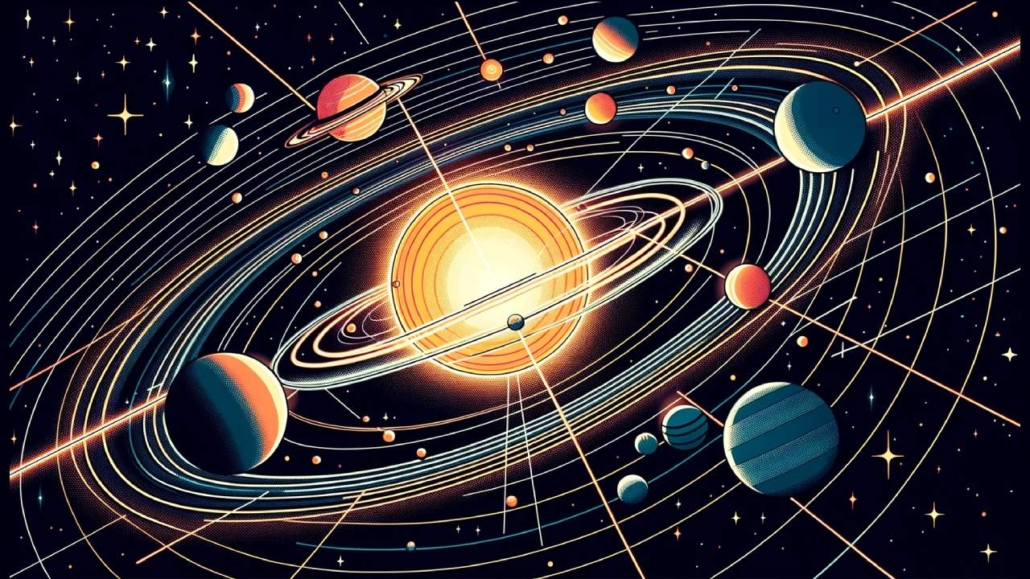
\includegraphics[width=0.5\linewidth]{portada}
		\label{fig:portada}
	\end{figure}
	
	\clearpage
	
	\begin{abstract}
		\begin{itemize}
			\item Esta aplicación ilustra cómo se usan las EDO para analizar un problema físico.
			
			\item Las leyes de Kepler se obtienen al conectar la ley de gravitación de Newton (expresada como una EDO) con el análisis del movimiento planetario en coordenadas polares.
			
			\item Los pasos de derivación de los vectores unitarios, velocidad y aceleración son esenciales para obtener las relaciones entre las cantidades involucradas en el movimiento.
			
			\item Este tipo de análisis es una piedra angular de la mecánica clásica y tiene implicaciones profundas en la comprensión del universo.
		\end{itemize}
	\end{abstract}
	
	\clearpage
	\tableofcontents  
	
	\clearpage
	
	\section{Introducción}
	Este material establece una conexión entre las leyes de Kepler y la ley de gravitación de Newton utilizando ecuaciones diferenciales. 

	• Problema: El objetivo de está aplicación es demostrar cómo la ley de gravitación de Newton (la fuerza que actúa sobre un planeta debido al Sol) conduce a las leyes de Kepler, que describen el movimiento planetario. Esto es históricamente inverso: Newton dedujo su ley a partir de las observaciones de Kepler. El punto aquí es ilustrar la conexión entre ambas mediante ED.

	\clearpage
	
	\section{Aplicación de los Sistemas de Primer Orden en Gravitación y las Leyes de Kepler.}
	
	A finales del siglo XVII, el astrónomo y matemático alemán Johannes Kepler analizó las detalladas observaciones planetarias recopiladas por el astrónomo Tycho Brahe y concluyó que el movimiento de los planetas alrededor del sol se describe por tres proposiciones formuladas por él, conocidas como las leyes de Kepler de movimiento planetario. 
	
	Las leyes de Kepler describen el movimiento de los planetas alrededor del Sol. Estas leyes revolucionaron la comprensión del movimiento planetario al demostrar que las órbitas de los planetas son elípticas y no circulares, como se creía antiguamente.
	
	Antes de Kepler, la teoría geocéntrica, que sostenía que el Sol y los planetas giraban alrededor de la Tierra, era ampliamente aceptada. Sin embargo, en el siglo XVI, Nicolás Copérnico propuso la teoría heliocéntrica, que afirmaba que los planetas giraban alrededor del Sol. Aunque esta teoría fue un avance significativo, todavía asumía que las órbitas eran circulares. Fue Kepler quien corrigió esta suposición y perfeccionó la teoría heliocéntrica con sus leyes del movimiento planetario.
	
	Las leyes de Kepler son leyes cinéticas. Esto quiere decir que su función es describir el movimiento planetario, cuyas características se deducen gracias a cálculos matemáticos. Con base en esta información, años más tarde Isaac Newton estudió las causas del movimiento de los planetas.
	
	\subsection{Leyes de Kepler:}
	
	\begin{itemize}
		\item Primera Ley: La órbita de cada planeta es una elipse con el Sol en uno de sus focos
		\item Segunda Ley: El radio vector desde el Sol hasta cada uno de los planetas recorre el área a una velocidad constante.
		\item Tercera Ley: El cuadrado del periodo de revolución del planeta es proporcional al cubo del semieje mayor de su órbita elíptica.
	\end{itemize}
	
	La primera ley de Kepler, también conocida como la \textbf{ley de las órbitas}, fue una revolución en la forma en que entendemos el movimiento planetario. Esta ley se aleja de la idea de que los planetas se mueven en círculos perfectos alrededor del Sol,  establece que los planetas se mueven en órbitas elípticas, con el Sol en uno de los focos de la elipse.
	
	Una elipse es una figura geométrica que se asemeja a un círculo estirado. A diferencia de un círculo, que tiene un centro único, una elipse tiene dos puntos focales. Para cualquier punto en la elipse, la suma de las distancias a los dos focos es constante.
	
	\begin{figure}
		\centering
		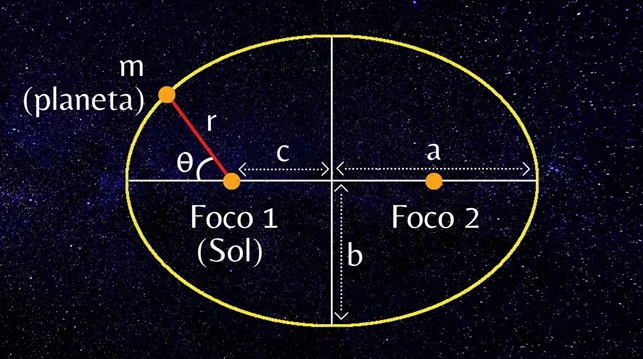
\includegraphics[width=0.6\linewidth]{elipse}
		\caption{Elipse \\ 
			     $\mathbf{\theta}$: ángulo.\\
			     a: semieje mayor.\\
		         b: semieje menor.\\
		         c: distancia focal o distancia del foco al centro.\\
		         r: radio vector o distancia entre el punto m (planeta) y el foco 1 (Sol).}
		\label{fig:elipse}
	\end{figure}
	
	
	\textbf{Ejemplos de la primera ley de kepler:}
	
	\underline{Órbita de la Tierra:} Aunque la órbita de la Tierra alrededor del Sol es casi circular, es ligeramente elíptica. Esto significa que hay un punto en el año, alrededor del 3 de enero, cuando la Tierra está más cerca del Sol (perihelio) y otro, alrededor del 4 de julio, cuando está más lejos (afelio). Sin embargo, la diferencia entre estas distancias es pequeña, lo que hace que la elipse de la Tierra sea casi circular.
	
	\underline{Órbita de Plutón:} A diferencia de la Tierra, Plutón tiene una órbita altamente elíptica. Esto significa que hay una variación significativa en su distancia al Sol durante su órbita. En el perihelio, Plutón puede estar más cerca del Sol que Neptuno, a pesar de que generalmente orbita más lejos.\\
	
	Mientras que la primera ley de Kepler se centró en la forma de la órbita, la segunda ley se adentra en cómo los planetas se mueven a lo largo de esa órbita, es decir, establece que el radio vector que une a un planeta con el Sol barre áreas iguales en tiempos iguales.
	
	El \textbf{radio vector} es una línea imaginaria que conecta el planeta con el Sol. A medida que el planeta se mueve en su órbita, este radio vector cambia de longitud y dirección, pero siempre barre áreas iguales en tiempos iguales.
	
	\begin{figure}[H]
		\centering
		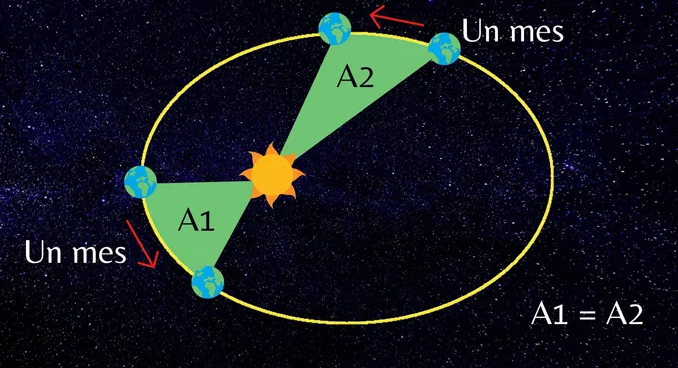
\includegraphics[width=0.6\linewidth]{radio_vector}
		\caption{Área recorrida por el radio vector.}
		\label{fig:radiovector}
	\end{figure}
	
	Se llama \textbf{velocidad areolar} al tiempo que demora un radio vector en recorrer áreas equivalentes. Ya que ese intervalo es siempre el mismo, se concluye que la velocidad areolar es constante.
	
	Esto implica que un planeta se moverá más rápido cuando esté más cerca del Sol y más lento cuando esté más lejos del Sol.
	
	Existen dos puntos en el recorrido de un planeta donde los cuerpos celestes alcanzan sus distancias y velocidades límites. Estos puntos se llaman perihelio y afelio.
	
	El perihelio es el punto más próximo de un planeta al Sol. En ese punto los planetas desarrollan su máxima velocidad.
	
	El afelio es el punto más lejano entre un planeta y el Sol. En ese punto los planetas alcanzan su velocidad mínima.
	
	\begin{figure}[H]
		\centering
		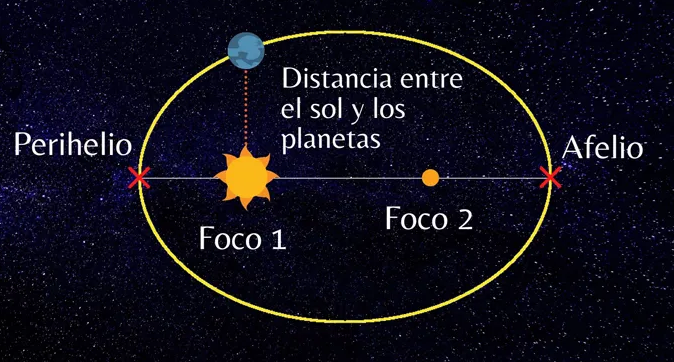
\includegraphics[width=0.6\linewidth]{segunda_ley}
		\caption{Movimiento de un planeta alrededor del Sol.}
		\label{fig:segundaley}
	\end{figure}
	
	
	La segunda ley de Kepler ayudo a entender que la fuerza gravitacional entre el Sol y un planeta no es constante, sino que varía dependiendo de la distancia entre ellos. Esta variación en la fuerza gravitacional es lo que causa la variación en la velocidad del planeta a medida que se mueve en su órbita.\\
	
	\textbf{Ejemplo de la segunda ley de kepler:}
	
	\underline{Cometas:} Los cometas, que a menudo tienen órbitas muy elípticas, ofrecen un ejemplo dramático de la segunda ley de Kepler en acción. Cuando un cometa se acerca al Sol, se mueve a velocidades increíblemente altas, y a medida que se aleja, su velocidad disminuye considerablemente.\\
	
	Después de establecer la forma de las órbitas y la naturaleza del movimiento planetario, Kepler se propuso encontrar una relación que vinculara las órbitas de todos los planetas conocidos en ese momento. Lo que descubrió fue una relación sorprendentemente simple entre el tamaño de la órbita de un planeta y el tiempo que tarda en completarla.
	
	Matemáticamente, la formula de la tercera ley de kepler se puede expresar como:
	
	\begin{equation*}
		T^2 = k * r^3
	\end{equation*}
	
	 donde:
	
	\begin{itemize}
		\item T es el período orbital del planeta (el tiempo que tarda en completar una órbita alrededor del Sol).
		\item r es el radio o el semieje mayor de la elipse orbital, que es esencialmente la distancia media del planeta al Sol.
		\item k (constante de proporcionalidad) es una constante que depende de la masa del Sol. 
	\end{itemize}
	
	Si dividimos el cuadrado del tiempo orbital entre el cubo del radio de la órbita, tendremos como resultado una constante, llamada constante de Kepler. La constante de Kepler es igual para todos los cuerpos celestes que orbitan alrededor del Sol, ya que no depende de ellos sino de la masa solar.
	
	\begin{equation*}
		\frac{\mathbf{T^2}}{\mathbf{r^3}} = k
	\end{equation*}
	
	Para ilustrar esta cuestión, en la siguiente tabla podemos comparar las características de todos los planetas, tomando en cuenta el período orbital (T) y el radio de órbita (r) para obtener la constante de Kepler (K). El período orbital se expresa en años, y el radio de órbita se expresa en unidades astronómicas (u.a). Veamos con atención el valor de K.
	
	\begin{table}[H]
		\centering
		\begin{tabular}{|c|c|c|c|} 
			\hline Planeta & T (años) & r (u.a) & K \\ 
			\hline Mercurio & 0.241 & 0.387 & 1.0002 \\ 
			\hline Venus & 0.615 & 0.723 & 1.000 \\ 
			\hline Tierra & 1 & 1 & 1.000 \\
			\hline Marte & 1.8881 & 1.524 & 0.999 \\
			\hline Júpiter & 11.86 & 5.204 & 0.997 \\
			\hline Saturno & 29.6 & 9.58 & 0.996 \\
			\hline Urano & 83.7 & 19.14 & 1.000 \\
			\hline Neptuno & 165.4 & 30.2 & 0.993 \\
			\hline 
	   \end{tabular}
	\end{table}
	
	Como podemos notar en la tabla, el valor de K es prácticamente el mismo para todos los planetas. La diferencia numérica es minúscula. Esto nos dice que, a pesar de las diferentes características de los planetas, la proporción es la misma. A esto llamamos la constante de Kepler.
	
	Está ley  proporcionó una forma simple y unificada de entender las órbitas de todos los planetas en el sistema solar. Además fue fundamental para el desarrollo de la ley de la gravitación universal de Newton, ya que sugiere una relación constante entre la distancia de un planeta al Sol y la fuerza gravitacional que actúa sobre él.\\
	
	\textbf{Ejemplo de la tercera ley de kepler:}
	
	\underline{Tierra y Marte:} La Tierra tiene un período orbital de 1 año y una distancia media al Sol de 1 unidad astronómica (UA). Marte, por otro lado, tiene un período orbital de aproximadamente 1,88 años y una distancia media al Sol de aproximadamente 1,52 UA. Si aplicamos la tercera ley de Kepler, encontramos que 1,882 es aproximadamente igual a 1,523, lo que confirma la ley.
	
	
	
	
	
	
	
	
	
	\clearpage
	\subsection{Ley de Gravitación Universal}
	Los principios de Newton son la obra más importante de la historia de la ciencia. En esta obra Newton exponía sus leyes de movimiento y su teoría de la gravedad. Una obra que le convertiría en el autor más importante de su era, y es posible que también de todos los tiempos.
	
	De la segunda Ley de Kepler que indica que el radio vector posición barre áreas iguales en tiempos iguales, se puede sacar la siguiente conclusión: el momento angular es constante a lo largo de toda la órbita, se conserva.
	
	Newton dedujo que existía una fuerza central gracias a esta segunda Ley de Kepler.
	
	Gracias a la Tercera dedujo que existía una fuerza que se movía con la inversa del cuadrado de la distancia.
	
	Teniendo en cuenta que es una fuerza que depende de la cantidad de materia, y usando las Leyes de Kepler, Newton descubrió la \textbf{ Ley de Gravitación Universal} la cual plantea que: Todos los cuerpos se atraen con una fuerza que es directamente proporcional al producto de sus masas e inversamente proporcional al cuadrado de la distancia que los separa. 
	
	Esta ley no sólo se aplica al movimiento de los planetas, sino a todos los cuerpos que existen en el universo, incluso a aquellos que se encuentran sobre la superficie terrestre.
	
	No obstante, el gran mérito de Newton fue demostrar que	a partir de la ley de gravitación universal , se pueden derivar matemáticamente las leyes de Kepler, es decir, Newton encontró una explicación teórica para las observaciones empíricas de Kepler, demostrando que estas leyes son una consecuencia natural de la atracción gravitacional entre los cuerpos. Este hecho constituyó una revolución no sólo científica sino también filosófica en la época.
	
	Matemáticamente la ley de gravitación de Newton se expresa:
	
	\begin{equation*}
		\mathbf{F} = G \frac{m_{1} m_{2}}{r^2}
	\end{equation*}
	
	Donde:
	
	\begin{itemize}
		\item F: es la magnitud de la fuerza gravitacional entre los dos cuerpos.
		\item G: es la constante de gravitación universal, $\mathbf{G}$ = $6.67384*10^-11 N*m^2/kg^2$, la cual no depende de las masas de los cuerpos.
		\item $m_{1}$: es la masa de uno de los cuerpos.
		\item $m_{2}$: es la masa de otro de los cuerpos.
		\item r: es la distancia entre los  centros de los cuerpos. (distancia que las separa)
	\end{itemize}
	
	Asumiendo que el Sol se localiza en el origen del plano de movimiento de un 
	planeta, y que escribimos el vector de posición del planeta en la forma:
	
	\begin{equation}
		\mathbf{r(t)} = (x(t),y(t)) = xi + yj
	\end{equation}
	
	
	donde $\mathbf{i}$ = $(1, 0)$  y $\mathbf{j}$ = $(0, 1)$ representan vectores unitarios en direcciones positivas $\mathbf{x}$ y $\mathbf{y}$ .Entonces, la ley de la gravitación del cuadrado inverso implica que el vector aceleración $\mathbf{r''(t)}$  del planeta esta dado por:
	
	
	\begin{equation}
		\mathbf{r''} = -\frac{kr}{r^3},
	\end{equation}
	
	donde $\mathbf{r}$  = $\sqrt{x^2 + y^2}$ es la distancia desde el sol hasta el planeta. Si las coordenadas polares del planeta en el tiempo $\mathbf{t}$ son $\mathbf{(x(t),\theta(t))}$, entonces los vectores unitarios radial y transversal estan dados por:
	
	\begin{equation} 
		\begin{aligned}
			\mathbf{u}_r = i \cos(\theta) + j \sin(\theta)  \quad \text{y} \quad \mathbf{u}_\theta = -i \sin(\theta) + j \cos(\theta) 
	    \end{aligned}
	\end{equation} 
	
	El vector unitario radial $\mathbf{u_{r}}$  (localizado en la posición del planeta) siempre apunta alejándose del origen, por tanto $\mathbf{u_{r}}$ = $\frac{\mathbf{r}}{r}$, y el vector unitario trasnversal $\mathbf{u_{\theta}}$ se obtiene a partir de $\mathbf{u_{r}}$ por una rotación de $90\degree$ 8 en sentido opuesto a las manecillas del reloj.
	
   \clearpage 
	
	\subsection{Realización de los pasos 1 - 4 necesarios para demostrar las Leyes de Kepler mediante la Ley de Gravitación.}
	\begin{itemize}
		\item \textbf{Paso 1:} Derive las ecuaciones en (3) término a término para mostrar que:
		
		\begin{equation} 
			\begin{aligned}
				\frac{d \mathbf{u}_r}{dt} = \mathbf{u}_\theta \frac{d\theta}{dt} \quad \text{y} \quad \frac{d \mathbf{u}_\theta}{dt} = \mathbf{-u}_r \frac{d\theta}{dt}
		    \end{aligned}
	   \end{equation} 
		
		\textbf{Solución:}
		
		\begin{equation*} 
			\mathbf{u}_r = i \cos(\theta) + j \sin(\theta) \tag{3}
		\end{equation*}
		
		\begin{equation*} 
			\frac{d \mathbf{u}_r}{dt} = \frac{d}{dt} \left( i \cos(\theta) + j \sin(\theta) \right)
		\end{equation*} 
		
		\begin{equation*}
			\frac{d \mathbf{u}_r}{dt} = \frac{d}{dt} \left( \cos(\theta) \right) \mathbf{i} + \frac{d}{dt} \left( \sin(\theta) \right) \mathbf{j}
		\end{equation*}
		
		\begin{equation*}
			\frac{d \mathbf{u}_r}{dt} = -\sin(\theta) \frac{d\theta}{dt} \mathbf{i} + \cos(\theta) \frac{d\theta}{dt} \mathbf{j}
		\end{equation*}
		
		\begin{equation*}
			\frac{d \mathbf{u}_r}{dt} = \frac{d\theta}{dt} \left( - \mathbf{i} \sin(\theta) + \mathbf{j} \cos(\theta) \right)
		\end{equation*}
		
		\begin{equation*}
			\frac{d \mathbf{u}_r}{dt} = \frac{d\theta}{dt} \mathbf{u}_\theta
		\end{equation*}
		
		Finalmente obtenemos la ec' (4):
		
		\begin{equation*}
			\frac{d \mathbf{u}_r}{dt} =  \mathbf{u}_\theta \ \frac{d\theta}{dt} \tag{4}
		\end{equation*}
	
	Pasamos para la segunda ec' :
	
	\begin{equation*}  
		\mathbf{u}_\theta = -i \sin(\theta) + j \cos(\theta) \tag{3}
	\end{equation*}
	
	\begin{equation*} 
		\frac{d \mathbf{u}_\theta}{dt} = \frac{d}{dt} \left( -i \sin(\theta) + j \cos(\theta) \right)
	\end{equation*} 
	
	\begin{equation*}
		\frac{d \mathbf{u}_\theta}{dt} = \frac{d}{dt} \left( -\sen(\theta) \right) \mathbf{i} + \frac{d}{dt} \left( \cos(\theta) \right) \mathbf{j}
	\end{equation*}
	
	\begin{equation*}
		\frac{d \mathbf{u}_\theta}{dt} = -\cos(\theta) \frac{d\theta}{dt} \mathbf{i}  -\sin(\theta) \frac{d\theta}{dt} \mathbf{j}
	\end{equation*}
	
	\begin{equation*}
		\frac{d \mathbf{u}_\theta}{dt} = \frac{d\theta}{dt} \left( - \mathbf{i} \cos(\theta) - \mathbf{j} \sin(\theta) \right)
	\end{equation*}
	
	\begin{equation*}
		\frac{d \mathbf{u}_\theta}{dt} = \frac{d\theta}{dt} - \left( \mathbf{i} \cos(\theta) + \mathbf{j} \sin(\theta) \right)
	\end{equation*}
	
	\begin{equation*}
		\frac{d \mathbf{u}_\theta}{dt} = \frac{d\theta}{dt} \mathbf{-u}_r
	\end{equation*}
	
	Finalmente la ec' (4):
	
	\begin{equation*}
		\frac{d \mathbf{u}_\theta}{dt} = \mathbf{-u}_r \frac{d\theta}{dt} \tag{5} 
	\end{equation*}
	
	\item \textbf{Paso 2:} Empléense las ecuaciones en (4) para derivar el vector de posición del planeta 
	\begin{equation*}
		\mathbf{r} = r \mathbf{u}_r
	\end{equation*}
	, y entonces muéstrese que su vector velocidad está dado por 
	
	\begin{equation}
		\mathbf{v} = \frac{d \mathbf{r}}{dt} = \mathbf{u}_r \frac{dr}{dt} + r \frac{d \theta}{dt} \mathbf{u}_\theta
	\end{equation}
	
	\textbf{Solución:}
	
	\begin{equation*}
		\frac{dr}{dt} = \frac{d}{dt}  \left( r \mathbf{u}_r \right)
	\end{equation*}
	
	\begin{equation*}
		\frac{dr}{dt} = \frac{dr}{dt} \mathbf{u}_r + r \frac{d \mathbf{u}_r}{dt}
	\end{equation*}
	
	Recordando que por (4) podemos sustituir:
	
	\begin{equation*}
		\frac{dr}{dt} = \frac{dr}{dt} \mathbf{u}_r + r \mathbf{u}_\theta \frac{d \theta}{dt}
	\end{equation*}
	
	reorganizando obtenemos la ec' (5):
	
	\begin{equation*}
		\frac{dr}{dt} = \mathbf{u}_r \frac{dr}{dt} + r \frac{d \theta}{dt} \mathbf{u}_\theta \tag{6}
	\end{equation*}
	
	\item \textbf{Paso 3:} Derive otra vez para demostrar que el vector aceleración del planeta
	
	\begin{equation*}
		\mathbf{a} = \frac{d \mathbf{v}}{dt}
	\end{equation*}
	
	está dado por 
	
	\begin{equation}
		\mathbf{a} = \left(\frac{d^2r}{dt^2} - r \left(\frac{d \theta}{dt}  \right)^2 \right) \mathbf{u}_r + \left(\frac{1}{r} \frac{d}{dt} \left( r^2 \frac{d \theta}{dt} \right) \right) \mathbf{u}_\theta
	\end{equation} 
	
	\textbf{Solución:}
	
	Como 
	
	\begin{equation*}
		\mathbf{v} = \frac{d \mathbf{r}}{dt} = \mathbf{u}_r \frac{dr}{dt} + r \frac{d \theta}{dt} \mathbf{u}_\theta
	\end{equation*}
	
	entonces, 
	
	\begin{equation*}
		\mathbf{a} = \frac{d}{dt} \left(\frac{dr}{dt} \mathbf{u}_r \right) + \frac{d}{dt} \left(r \frac{d \theta}{dt} \mathbf{u}_\theta \right)
	\end{equation*}
	
	
	\begin{equation*}
		\mathbf{a} = \frac{d^2r}{dt^2} \mathbf{u}_r + \frac{dr}{dt} \frac{d \mathbf{u}_r}{dt}  + \frac{dr}{dt} \frac{d \theta}{dt} \mathbf{u}_\theta + r \frac{d^2\theta}{dt^2} \mathbf{u}_\theta + r \frac{d \theta}{dt} \frac{d \mathbf{u}_\theta}{dt}
	\end{equation*}
	
	Sustituyendo las ecuaciones en (4) obtenemos:
	
	\begin{equation*}
		\mathbf{a} = \frac{d^2r}{dt^2} \mathbf{u}_r + \frac{dr}{dt} \frac{d \theta}{dt} \mathbf{u}_\theta + \frac{dr}{dt} \frac{d \theta}{dt} \mathbf{u}_\theta + r \frac{d^2\theta}{dt^2} \mathbf{u}_\theta + r \frac{d \theta}{dt} \left( -\mathbf{u}_r \frac{d \theta}{dt} \right)
	\end{equation*}
	
	\begin{equation*}
		\mathbf{a} = \frac{d^2r}{dt^2} \mathbf{u}_r + \frac{dr}{dt} \frac{d \theta}{dt} \mathbf{u}_\theta + \frac{dr}{dt} \frac{d \theta}{dt} \mathbf{u}_\theta +  r \frac{d^2\theta}{dt^2} \mathbf{u}_\theta - r \left(\frac{d \theta}{dt} \right)^2 \mathbf{u}_r
	\end{equation*}
	
	\begin{equation*}
		\mathbf{a} = \left(\frac{d^2r}{dt^2} - r \left(\frac{d \theta}{dt} \right)^2 \right) \mathbf{u}_r + \left(2 \frac{dr}{dt} \frac{d \theta}{dt} + r \frac{d^2\theta}{dt^2} \right) \mathbf{u}_\theta  \tag{6'}
	\end{equation*}
	
	Como la expresión,
	
	\begin{equation*}
		\frac{d}{dt} \left(r^2 \frac{d \theta}{dt} \right) = 2r \frac{dr}{dt} \frac{d \theta}{dt} + r^2 \frac{d^2\theta}{dt^2}
	\end{equation*}
	
	entonces,
	
	\begin{equation*}
		\frac{1}{r} \frac{d}{dt} \left(r^2 \frac{d \theta}{dt} \right) = \frac{1}{r} \left(2r \frac{dr}{dt} \frac{d \theta}{dt} + r^2 \frac{d^2\theta}{dt^2} \right)
	\end{equation*}
	
	de la multiplicación resultante obtenemos;
	
	\begin{equation*}
		\frac{1}{r} \frac{d}{dt} \left(r^2 \frac{d \theta}{dt} \right) = \left(2 \frac{dr}{dt} \frac{d \theta}{dt} + r \frac{d^2\theta}{dt^2} \right)
	\end{equation*}
	 
	 por tanto, la ecuación (6') se puede reescribir como,
	 
	 \begin{equation*}
	 		\mathbf{a} = \left(\frac{d^2r}{dt^2} - r \left(\frac{d \theta}{dt} \right)^2 \right) \mathbf{u}_r +  \left(\frac{1}{r} \frac{d}{dt} \left(r^2 \frac{d \theta}{dt} \right) \right) \mathbf{u}_\theta
	 \end{equation*}
	
	\item \textbf{Paso 4:} Las componentes radial y transversal en los lados derechos de las ecuaciones (2) y (6) deben coincidir. Igualando las componentes transversales esto es, los coeficientes de $\mathbf{u}_\theta$ se obtiene,
	
	\begin{equation}
		\frac{1}{r} \frac{d}{dt} \left( r^2 \frac{d \theta}{dt} \right) = 0
	\end{equation}
	
	por tanto se sigue que,
	
	\begin{equation}
		r^2 \frac{d \theta}{dt} = h
	\end{equation}
	
	donde h es una constante
	
	\textbf{Igualando las componentes transversales de las ecuaciones (2) y (6)}
	
	\begin{equation*}
		\frac{1}{r} \frac{d}{dt} \left(r^2 \frac{d \theta}{dt} \right) = 0
	\end{equation*}
	
	En la ley de gravitación universal no hay presencia de fuerza transversal ($\mathbf{u}_\theta$) por ende, la componente transversal de la ecuación (2) en este caso es cero.
	
	Asumiendo que el vector acelaración $\mathbf{r \neq 0}$ multiplicamos y obtenemos:
	
	\begin{equation*}
		\frac{d}{dt} \left(r^2 \frac{d \theta}{dt} \right) = 0
	\end{equation*}
	
	y por tanto ,
	
	\begin{equation*}
		r^2 \frac{d \theta}{dt} = h
	\end{equation*}
	\end{itemize}
	
	\clearpage
	
	\section{Conclusiones}
	Este trabajo demuestra cómo las ecuaciones diferenciales ordinarias (EDO) conectan la Ley de Gravitación Universal de Newton con las Leyes de Kepler, permitiendo comprender el movimiento planetario desde un enfoque matemático riguroso. Es impresionante ver cómo estas ecuaciones, a través de derivaciones de vectores de posición, velocidad y aceleración, respaldan las observaciones empíricas de Kepler y las explican como una consecuencia natural de la gravitación universal. Esto no solo refuerza la importancia de las EDO en la física clásica, sino que también resalta su capacidad para modelar fenómenos complejos y unificar teoría y observación. En definitiva, este análisis es un ejemplo claro de cómo las matemáticas son esenciales para entender y predecir el comportamiento del universo.\\
	
	\section{Bibliografía}
	
	”Differential Equations and Boundary Value Problems:
	Computing and Modeling, 4th Edition”, de C. Henry Edwards and David E. Penney.
	 
\end{document}
